\documentclass[conference]{IEEEtran}
\IEEEoverridecommandlockouts
\usepackage{cite}
\usepackage{amsmath,amssymb,amsfonts,amsthm}
\usepackage{graphicx}
\usepackage{booktabs}
\usepackage{multirow}
\usepackage{xcolor}
\usepackage{url}
\usepackage[hidelinks]{hyperref}
\newcommand{\jbr}{\mathrm{JBR}}
\newtheorem{proposition}{Proposition}
\graphicspath{{figures/}}

\begin{document}

\title{When Does Pooling Fail at a Foreign-Key Join? A Validated Capacity Law for Learned Aggregation in Relational Deep Learning}

\author{\IEEEauthorblockN{Vasu Atmakuri}
\IEEEauthorblockA{\textit{Independent Researcher}\\
Dallas, TX, USA \\
athmakurivasu@gmail.com}}

\maketitle

\begin{abstract}
Relational deep learning trains graph neural networks directly on multi-table databases, and every foreign-key join is resolved by a learned aggregation that compresses a variable-size set of child rows into a fixed-width parent embedding. We characterize when this compression fails, in 8{,}150 controlled training runs and 704 runs on RelBench databases. On set-dependent targets, accuracy of sum and mean aggregation falls along a sigmoid in the Join Bottleneck Ratio, $\jbr = K H_{\mathrm{row}}/d$ (child cardinality times row entropy over embedding width), with $R^2 = 0.87$ to $0.95$. The ratio is right in cardinality but wrong in width: a corrected law, $K H_{\mathrm{row}}^{0.9}/d^{0.2}$, fitted on 76 configurations and frozen before new runs, predicts accuracy on 36 unseen configurations with $R^2 = 0.86$ and $0.89$, against $0.49$ for the original ratio, and its exponents transfer to message-passing models ($R^2 = 0.76$ against $0.58$). Two mechanisms move the threshold where width does not: attention with the parent as query tolerates $3.8$ times larger joins, and a second message-passing layer gives sum aggregation a $2.8$ to $3.2$ times gain, but only when the parent first sends a message to its children. On real RelBench tables with planted labels, the same law appears: accuracy on labels that require one specific child row falls from $0.97$ to $0.64$ on average as the number of children grows from 4 to 64, attention with two layers retains $0.88$, and count-type labels stay at $1.00$ for every aggregator. On twelve original RelBench tasks, by contrast, replacing sum with a fairly implemented attention changes AUROC by $-0.4$ points (95\% CI $[-1.6, 0.6]$), widening from 32 to 512 changes it by $-0.1$ points, and three times longer training leaves both conclusions unchanged; the ratio also does not predict published task difficulty, although 44 of 95 foreign keys exceed it. The bottleneck is real and predictable, but current benchmark labels rarely depend on the information it removes.
\end{abstract}

\begin{IEEEkeywords}
relational deep learning, graph neural networks, set aggregation, capacity law, relational databases, RelBench, attention
\end{IEEEkeywords}

\section{Introduction}

Most enterprise data lives in relational databases, where the signal needed for a prediction about one entity is spread across many tables. Relational deep learning (RDL) \cite{fey2024relational} turns the database into a heterogeneous temporal graph, with one node per row and one edge per primary-key/foreign-key link, and trains a graph neural network end to end. RelBench \cite{robinson2024relbench} made this practical and comparable, and newer architectures such as RelGNN \cite{chen2025relgnn} and the Relational Graph Transformer \cite{dwivedi2025relgt} have improved on the original pipeline.

In every such model, a parent row receives messages from all of its child rows across a foreign key and must combine them into one fixed-width vector: a customer with $K$ transactions of $D$ columns becomes one $d$-dimensional embedding. Feature engineering \cite{kanter2015dfs} makes this reduction explicit with counts and means; RDL learns it, but the width stays fixed. Theory on set functions shows that sum decompositions need latent width on the order of the set size to be injective \cite{wagstaff2019limitations,wagstaff2022universal}, and work on over-squashing shows that fixed-width messages can bottleneck graph networks \cite{alon2021bottleneck,topping2022oversquashing,digiovanni2023oversquashing}. These results are worst-case or asymptotic. A practitioner needs quantitative answers to narrower questions:
(Q1) at what ratio of incoming information to width does learned pooling stop working;
(Q2) which variables control that threshold, and can it be predicted for a join that was never tested;
(Q3) which design choices move it;
(Q4) does the same behavior appear on real database tables; and
(Q5) does it limit accuracy on current benchmarks?

\textbf{Contributions.}
\begin{itemize}
\item A controlled study of 8{,}150 synthetic training runs over 147 join configurations, with per-configuration learning-rate selection, and 704 runs on four RelBench databases.
\item A capacity law. Accuracy follows a sigmoid in the Join Bottleneck Ratio ($R^2 = 0.87$ to $0.95$), but the ratio over-credits width. A corrected law with exponents $0.9$ on entropy and $0.2$ on width was frozen before new experiments and then predicted 36 unseen configurations with $R^2 = 0.86$ to $0.89$, versus $0.49$ for the original ratio; a second pre-registered test shows that the exponents transfer to message-passing models.
\item Mechanisms, with short formal arguments: parent-conditioned attention ($3.8\times$) and a parent-to-child message before pooling ($2.8$ to $3.2\times$) move the threshold; width ($d^{0.2}$) and depth without that message do not.
\item Confirmation on real tables: planted labels on RelBench tables, selected by a pre-declared inclusion rule and run with three seeds, reproduce the decline with cardinality and the benefit of both mechanisms, while count-type labels are unaffected.
\item An answer to Q5: on twelve RelBench tasks, aggregation choice and width barely change accuracy once attention is implemented fairly, and the ratio does not predict task difficulty, although about half of all foreign keys exceed it. We also identify an implementation detail of the stock heterogeneous attention layer that accounts for most of the apparent disadvantage of attention on these tasks.
\end{itemize}

\section{Related Work}

\textbf{Relational deep learning.} Learning directly on relational databases was argued for in \cite{cvitkovic2020supervised} and formalized as RDL in \cite{fey2024relational}. RelBench \cite{robinson2024relbench} provides temporal splits, entity and recommendation tasks, and baselines comparing a GraphSAGE-based model \cite{hamilton2017graphsage} with LightGBM \cite{ke2017lightgbm} on engineered features. RelGNN \cite{chen2025relgnn} adds composite message passing through bridge tables, and RelGT \cite{dwivedi2025relgt} adds attention over sampled subgraphs.

\textbf{Expressivity of aggregation.} Deep Sets \cite{zaheer2017deepsets} established sum decompositions as universal for set functions, and continuous sum decompositions require latent dimension at least equal to the set size \cite{wagstaff2019limitations,wagstaff2022universal}. Graph Isomorphism Networks \cite{xu2019gin} motivated sum over mean and max, and Principal Neighbourhood Aggregation \cite{corso2020pna} combined several aggregators. Attention \cite{velickovic2018gat,brody2022gatv2,lee2019settransformer} and Janossy pooling \cite{murphy2019janossy} can select instead of summarize. We measure what is learned at finite width and budget.

\textbf{Bottlenecks and empirical laws.} Over-squashing \cite{alon2021bottleneck,topping2022oversquashing,digiovanni2023oversquashing} describes receptive fields compressed into fixed-width vectors, with width as one proposed remedy \cite{digiovanni2023oversquashing}. Empirical scaling laws \cite{hestness2017scaling,kaplan2020scaling} show that simple power laws can be measured and extrapolated when experiments are controlled; we follow that methodology for one relational operation and add a pre-registered out-of-sample test.

\section{The Join Bottleneck Ratio}

For a foreign key from a child table to a parent table, let a parent have $K$ linked child rows of $D$ columns, and let a learned aggregator map them to $\mathbf{h}_p \in \mathbb{R}^d$. With $H_{\mathrm{row}} = \sum_j H(x_j)$ the summed plug-in entropy of the child columns in bits, an upper bound on the joint row entropy \cite{cover2006elements}, we define
\begin{equation}
\jbr = \frac{K\,H_{\mathrm{row}}}{d}.
\label{eq:jbr}
\end{equation}
The ratio counts incoming bits per embedding dimension. It is not a Shannon capacity, since a real coordinate can in principle store unbounded information; the hypothesis is that gradient-trained aggregators have a bounded effective capacity per dimension. We also use the multiset ratio $\jbr_{\mathrm{set}} = \log_2\binom{2^{H_{\mathrm{row}}}+K-1}{K}/d$, the effective ratio $\jbr_{\mathrm{eff}} = K(H_{\mathrm{row}} + H_{\mathrm{lookup}})/d$ that adds the entropy of the child's own lookup parents, and the generalized form
\begin{equation}
\log_2 X = \log_2 K + a_H \log_2 H_{\mathrm{row}} - a_d \log_2 d,
\label{eq:law}
\end{equation}
which reduces to \eqref{eq:jbr} when $a_H = a_d = 1$.

\textbf{Why pooling and selection scale differently.} Three short arguments explain the shape of the results that follow. Consider the parent-query existence task used throughout: does some child row equal a value $q$ carried by the parent?

\begin{proposition}[pooled codes]
Let each child value be encoded by an independent random vector $\phi(x) \in \{\pm d^{-1/2}\}^d$ and pooled by summation, $s = \sum_{i=1}^K \phi(x_i)$. The statistic $T = \langle s, \phi(q)\rangle$ has mean $1$ if $q$ occurs once and $0$ if it does not, with interference variance $(K-1)/d$ or $K/d$. A fixed error rate therefore requires $d \ge c K$.
\end{proposition}
\noindent\emph{Sketch.} Cross terms $\langle \phi(x_i), \phi(q) \rangle$ for $x_i \neq q$ are independent, zero-mean, with variance $1/d$; the two classes are separated by a unit shift against noise of standard deviation $\sqrt{K/d}$. \qed

Ideal codes thus need width proportional to $K$, with no dependence on $H_{\mathrm{row}}$ beyond the requirement that codes be distinct. A learned encoder must instead discover near-orthogonal codes for up to $2^{H_{\mathrm{row}}}$ values from data, which is where entropy enters, and our measurements show that gradient training converts extra width into capacity far less efficiently than random codes would ($a_d \approx 0.2$).

\begin{proposition}[selection]
If attention scores satisfy $\langle W_Q \mathbf{h}_p, W_K \mathbf{h}_i \rangle = \beta$ for the matching child and at most $\beta\varepsilon$ otherwise, the attention weight on the match is at least $(1 + (K-1)e^{-\beta(1-\varepsilon)})^{-1}$, which stays near one when $\beta(1-\varepsilon) \ge \log K$.
\end{proposition}
\noindent\emph{Sketch.} Direct from the softmax. \qed

Selection replaces width linear in $K$ by a score scale logarithmic in $K$; width is still needed to separate the query from the other values, which is why attention also fails when $d$ is very small.

\begin{proposition}[message before pooling]
If each child first receives $\mathbf{h}_p$ and computes $g(x_i, q) = \mathbb{1}[x_i = q]$, then $\sum_i g$ answers the task with one dimension for any $K$, whereas $\frac{1}{K}\sum_i g$ separates the classes only by $1/K$.
\end{proposition}

A parent-to-child message turns a summarization problem into a counting problem, which pooling solves well, and sum benefits more than mean.

\section{Experimental Design}
\label{sec:design}

\subsection{Synthetic relational data}

Each parent has a query $\mathbf{q}_p \in \{0,1\}^D$ and $K$ child rows of $D$ uniform bits, so $H_{\mathrm{row}} = D$. \emph{Mean-based}: $y = \mathbb{1}[\mathbf{w}^\top(\bar{\mathbf{x}} - \tfrac12) > 0]$ for a fixed direction $\mathbf{w}$, a control that needs only the first moment. \emph{Rare pattern}: $y = 1$ if exactly one child equals $\mathbf{q}_p$ and $0$ if none does. \emph{Distributional}: $y = 1$ if $\mathbf{q}_p$ appears twice and $0$ if once. Non-planted rows that collide with $\mathbf{q}_p$ are moved off it by one bit flip, so the classes cannot be separated by marginal statistics. Training batches are generated fresh at every step; validation and test sets are fixed samples from separate streams.

\textbf{Configurations.} A core grid of 25 configurations at $d = 128$ spans $\jbr$ from $1/32$ to $16$, including five decompositions at $\jbr = 1$, $(K, D) \in \{(4,32), (8,16), (16,8), (32,4), (64,2)\}$. An architecture subset has 11 configurations, an extended range 63 configurations up to $\jbr = 4096$ (by varying $d$ from 4 to 128), and a width sweep seven $(K,D)$ pairs at $d = 4$ to $512$. For the out-of-sample test, 36 configurations with $K \in \{3, 6, \dots, 96\}$, $D \in \{3, 6, 12, 24\}$ and $d \in \{24, 48, 96, 192\}$ were selected by a fixed rule to cover $\log_2\jbr$ from $-3$ to $5$; none shares a value of $K$, $D$ or $d$ with the fitting data.

\subsection{Models and training}

\textbf{DeepSets} \cite{zaheer2017deepsets}: per-child encoder MLP to width $d$, sum, mean or max pooling, concatenation with a parent encoding, decoder MLP, hidden width $\max(128, d)$. \textbf{One message-passing layer}: $\mathbf{h}_p' = \sigma(W_s \mathbf{h}_p + \mathrm{AGG}_i\, W_m \mathbf{h}_i)$ with sum, mean, or multi-head attention with the parent as query (1 or 4 heads). \textbf{Two layers}: a parent-to-child layer $\mathbf{h}_i' = \sigma(W_c \mathbf{h}_i + W_{pc}\mathbf{h}_p)$ followed by the pooling layer; the control replaces the first layer by a child-only layer of equal depth.

Adam, batch 128, 4{,}000 to 8{,}000 steps, validation AUROC every 200 steps with patience 10, test AUROC at the best validation checkpoint, three seeds (two for the out-of-sample test). For every configuration and seed the learning rate is selected on validation AUROC from $\{10^{-4}, 3\cdot10^{-4}, 10^{-3}\}$ (for the out-of-sample and two-layer runs from $\{3\cdot10^{-4}, 10^{-3}\}$, adding $10^{-4}$ at $d \ge 192$). All runs used two laptops without a GPU.

\subsection{Statistics}

For each family, target and model we fit $\mathrm{AUROC} = a + (b-a)/(1 + e^{s(x - m)})$ over configuration means, with $x = \log_2\jbr$ or the predictor of \eqref{eq:law}, and report $R^2$ and the midpoint $m$. The capacity multiplier of a model is $2^{m - m_{\mathrm{sum}}}$. Intervals are bootstrap intervals over seeds within configurations, or over configurations for the out-of-sample comparison. The out-of-sample predictions were computed from frozen fits and committed to the public repository before the new runs started; the commit time is the pre-registration record. For RelBench predictors we use Spearman correlation with permutation tests within databases, within-database concordance, leave-one-database-out (LODO) $R^2$, and Holm correction \cite{holm1979}.

\section{Results on Controlled Data}

\begin{figure*}[t]
\centering
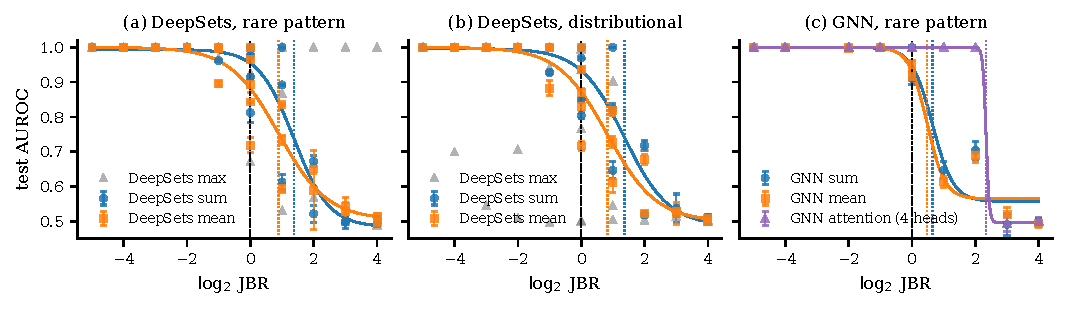
\includegraphics[width=\textwidth]{phase_transition.pdf}
\caption{Test AUROC against $\log_2\jbr$ after learning-rate selection (points: configuration means over three seeds; bars: one standard deviation; curves: sigmoid fits; dotted lines: midpoints). Sum and mean follow a sigmoid on both set targets; max does not. In (c), four-head attention stays near 1.0 well past the transition of sum and mean.}
\label{fig:phase}
\end{figure*}

\subsection{Q1: a sigmoid transition near $\jbr \approx 2$}

For both set targets and both sum and mean, in both families, a sigmoid in $\log_2\jbr$ explains $87\%$ to $95\%$ of the variance (mean $R^2 = 0.916$, 95\% CI $[0.896, 0.933]$, nine fits; Fig.~\ref{fig:phase}, Table~\ref{tab:fits}). Below $\jbr = 0.5$ mean AUROC is at least $0.989$ in every fit; above $\jbr = 2$ it is $0.53$ to $0.58$, and above $\jbr = 4$ it is $0.50$ to $0.52$, which is chance. Midpoints lie at $\jbr \approx 1.8$ to $2.6$ for DeepSets and $1.4$ to $1.6$ for one message-passing layer. The mean-based control stays between $0.99$ and $1.00$ for sum and mean at every ratio, and max pooling does not follow the law ($R^2 = 0.28$ and $0.32$). At equal ratio, the five decompositions at $\jbr = 1$ give AUROC coefficients of variation of $0.08$ to $0.10$ for sum and $0.12$ to $0.13$ for mean.

The threshold depends on optimization: at a fixed learning rate of $10^{-3}$ the same fits put the midpoints near $\jbr = 1$, and per-configuration selection moves them up by a factor of $1.8$ to $2.6$, mostly by choosing smaller rates for wide encoders ($10^{-4}$ in $81\%$ of cases at $d = 512$). A larger step budget helps far less (for example $0.846$ to $0.934$ at $K = 8, D = 8$ from half to four times the budget, and nothing for $K \ge 32$).

\begin{table}[t]
\caption{Sigmoid fits of test AUROC on $\log_2\jbr$ (set targets, learning rate selected per configuration).}
\label{tab:fits}
\centering
\setlength{\tabcolsep}{4pt}
\begin{tabular}{llcccc}
\toprule
Family & Target & Model & $R^2$ & $m$ & $\jbr$ at $m$\\
\midrule
DeepSets & rare pattern & sum & 0.882 & 1.37 & 2.58\\
DeepSets & rare pattern & mean & 0.900 & 0.89 & 1.85\\
DeepSets & distributional & sum & 0.869 & 1.36 & 2.57\\
DeepSets & distributional & mean & 0.902 & 0.83 & 1.78\\
GNN, 1 layer & rare pattern & sum & 0.930 & 0.65 & 1.56\\
GNN, 1 layer & rare pattern & mean & 0.948 & 0.47 & 1.39\\
GNN, 1 layer & distributional & sum & 0.938 & 0.61 & 1.52\\
GNN, 1 layer & distributional & mean & 0.949 & 0.50 & 1.41\\
\midrule
GNN, 2 layers & rare pattern & sum & 0.919 & 2.13 & 4.39\\
GNN, 2 layers & distributional & sum & 0.901 & 2.27 & 4.84\\
Extended & rare pattern & sum & 0.930 & 1.50 & 2.83\\
Extended & rare pattern & attn (1h) & 0.771 & 3.44 & 10.86\\
Extended & rare pattern & attn (4h) & 0.810 & 3.08 & 8.43\\
\bottomrule
\end{tabular}
\end{table}

\subsection{Q2: a corrected law that predicts unseen joins}

\begin{figure}[t]
\centering
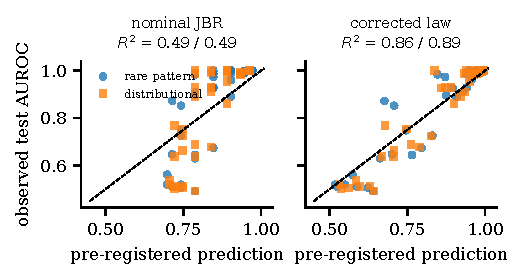
\includegraphics[width=\columnwidth]{out_of_sample_validation.pdf}
\caption{Pre-registered out-of-sample test on 36 configurations not used for fitting. Left: the original ratio. Right: the corrected law \eqref{eq:law}. Each point is one configuration and target; the dashed line is perfect prediction.}
\label{fig:oos}
\end{figure}

Fitting \eqref{eq:law} on all 76 DeepSets-sum configurations of the core grid and width sweep gives $a_H = 0.92$ and $a_d = 0.22$ (rare pattern) and $a_H = 0.90$, $a_d = 0.21$ (distributional), with in-sample $R^2 = 0.73$ and $0.70$, against $0.49$ and $0.45$ for the original ratio on the same configurations. Cardinality and entropy enter almost as the ratio assumes; width does not. Doubling $d$ raises the tolerated cardinality by only $2^{0.2} \approx 1.15$.

We froze these fits, together with a fit of the multiset ratio, and predicted AUROC for 36 new configurations before running them. Fig.~\ref{fig:oos} and Table~\ref{tab:oos} show the outcome. The corrected law predicts the unseen configurations with $R^2 = 0.86$ and $0.89$ and a mean absolute error of $0.05$ AUROC; the original ratio reaches $0.49$ with an error of $0.12$, and the multiset ratio is worse still. The improvement in $R^2$ is $0.37$ (95\% CI $[0.28, 0.49]$) and $0.40$ ($[0.32, 0.51]$). The largest misses of the corrected law are configurations with small $D$ and large $K$ (for example $K = 96$, $D = 3$), where only eight row values exist and pooling behaves more like a histogram; these are underpredicted, consistent with Proposition 1.

A second pre-registered test asks whether the exponents are specific to DeepSets. We kept $a_H$ and $a_d$ from the DeepSets fit, refitted only the sigmoid on 63 one-layer message-passing configurations, and predicted the same 36 new configurations for message passing with sum aggregation (three seeds). The transferred law reaches $R^2 = 0.76$ (mean absolute error $0.066$) against $0.58$ ($0.085$) for the original ratio, and exponents refitted on message-passing data ($a_H = 1.06$, $a_d = 0.29$) do barely better ($0.77$). The improvement over the original ratio is smaller than for DeepSets and its interval touches zero ($+0.18$, 95\% CI $[-0.01, 0.45]$), but the direction and the weak width exponent carry over.

\begin{table}[t]
\caption{Pre-registered prediction of 36 unseen configurations (test AUROC). Top: DeepSets sum. Bottom: the exponents fitted on DeepSets, transferred to message passing.}
\label{tab:oos}
\centering
\setlength{\tabcolsep}{4pt}
\begin{tabular}{lcccc}
\toprule
& \multicolumn{2}{c}{Rare pattern} & \multicolumn{2}{c}{Distributional}\\
Predictor & $R^2$ & MAE & $R^2$ & MAE\\
\midrule
Original $\jbr$ & 0.487 & 0.115 & 0.486 & 0.115\\
Multiset $\jbr_{\mathrm{set}}$ & 0.379 & 0.131 & 0.340 & 0.137\\
Corrected law \eqref{eq:law} & \textbf{0.856} & \textbf{0.049} & \textbf{0.891} & \textbf{0.048}\\
\midrule
\multicolumn{5}{l}{\emph{One-layer message passing, sum (rare pattern)}}\\
Original $\jbr$ & 0.576 & 0.085 & & \\
Law, DeepSets exponents & \textbf{0.761} & \textbf{0.066} & & \\
\bottomrule
\end{tabular}
\end{table}

\subsection{Q3: what moves the threshold}

\begin{figure}[t]
\centering
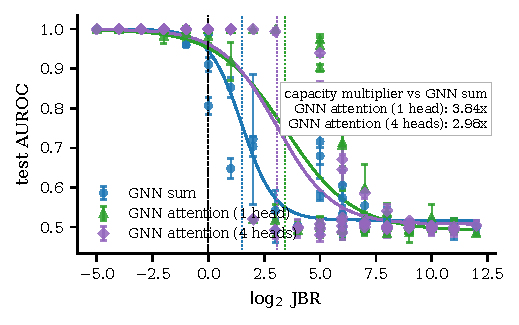
\includegraphics[width=\columnwidth]{capacity_multiplier.pdf}
\caption{Extended range ($\jbr$ up to 4096). Attention with the parent as query shifts the transition of sum aggregation by a factor of 3.84 (one head) and 2.98 (four heads).}
\label{fig:mult}
\end{figure}

\textbf{Selection.} On the extended range (Fig.~\ref{fig:mult}), single-head attention moves the midpoint from $\log_2\jbr = 1.50$ to $3.44$, a capacity multiplier of $3.84$ (95\% CI $[3.29, 4.40]$); four heads give $2.98$ ($[2.53, 3.40]$), since splitting $d$ across heads reduces the per-head width. Attention curves fit less well ($R^2 = 0.77$ and $0.81$) because at very small $d$ the query and child codes no longer fit in the head dimension, as Proposition 2 anticipates.

\textbf{A message before pooling.} With a second layer in which children first receive the parent's embedding, sum aggregation moves its midpoint from $0.65$ to $2.13$ (rare pattern; 95\% CI of the two-layer midpoint $[2.07, 2.21]$) and from $0.61$ to $2.27$ (distributional), a multiplier of $2.8$ to $3.2$, close to that of attention (Fig.~\ref{fig:depth}). The same depth without the parent-to-child message gives no gain (midpoints $0.38$ and $0.33$), and mean aggregation gains nothing from the message ($0.57$ and $0.55$). This is the pattern of Proposition 3: the message lets each child test itself against the query, and only summation turns the resulting indicators into a count that does not shrink with $K$. Above $\jbr = 8$ all models are at chance.

\begin{figure}[t]
\centering
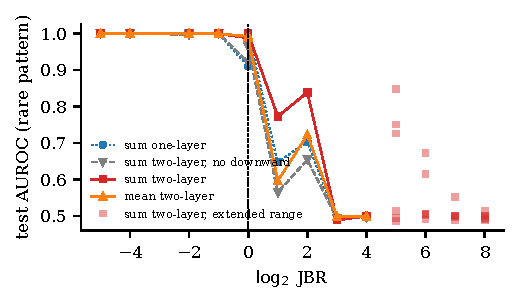
\includegraphics[width=\columnwidth]{depth.pdf}
\caption{Two message-passing layers, rare pattern target. With the parent-to-child message, sum aggregation tolerates about three times larger ratios; without it, depth alone does not help.}
\label{fig:depth}
\end{figure}

\textbf{Width} is the weak lever. Under the fitted exponent, matching the attention multiplier by widening a sum aggregator would require roughly $2^{1.94/0.2} \approx 800$ times more width.

\subsection{Robustness}

\begin{figure*}[t]
\centering
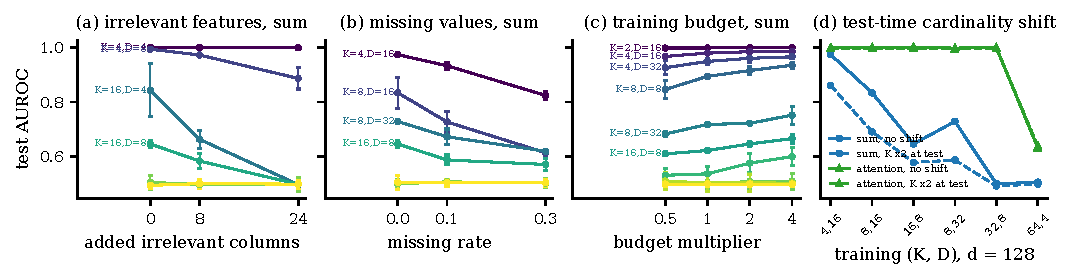
\includegraphics[width=\textwidth]{controls.pdf}
\caption{Controls (DeepSets sum unless stated, $d = 128$, three seeds). (a) Irrelevant child columns consume capacity. (b) Missing values degrade accuracy steadily. (c) A four times larger budget gives modest gains below the transition and none above it. (d) Doubling $K$ at test time hurts sum aggregation; attention is unaffected until $K = 64$.}
\label{fig:controls}
\end{figure*}

Fig.~\ref{fig:controls} summarizes the controls. Adding 24 irrelevant columns lowers sum aggregation at $K = 16, D = 8$ from $0.647$ to $0.500$ and attention from $0.999$ to $0.951$, so the entropy that matters is what the encoder cannot cheaply discard. Missing rates of $0.1$ and $0.3$ lower AUROC from $0.973$ to $0.933$ and $0.824$ at $K = 4, D = 16$. Doubling $K$ at test time lowers sum aggregation from $0.834$ to $0.691$ at $K = 8, D = 16$, while attention stays at or above $0.994$ up to $K = 32$.

\section{Results on RelBench}

\subsection{Q4: the law on real tables}

\begin{figure}[t]
\centering
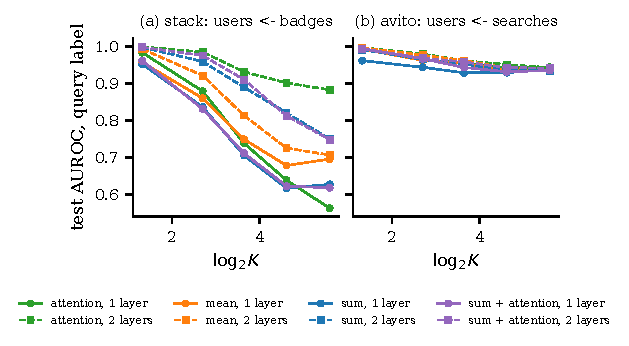
\includegraphics[width=\columnwidth]{planted_signal_by_children.pdf}
\caption{Planted query labels on real RelBench tables ($d = 128$): test AUROC within bins of the number of admissible children $K$ of each test entity. Joins selected by the pre-declared inclusion rule. Count-type labels on the same tables (not shown) reach 1.000 for every aggregator.}
\label{fig:planted}
\end{figure}

To test the mechanism on real data with a known ground truth, we keep real RelBench tables, cardinalities and child features and plant only the label. For a join from a child table to an entity table, one child column is chosen by a fixed rule (the discrete column with most distinct values, hashed into at most 1{,}000 buckets), and each entity receives a categorical column holding a query value. The \emph{query label} is 1 if some child visible at the seed time carries the entity's query value. The \emph{count label} is 1 if some visible child carries one of a fixed set of common values, the same for every entity. Both labels share the same graph and inputs. Seeds and timestamps come from a RelBench task on the entity table, restricted to entities with 1 to 64 visible children so that the sampler (fanout 64) always sees all of them. We train the standard RelBench RDL pipeline (Section~\ref{sec:real}) with one or two layers and four aggregations.

Before the final runs we fixed an inclusion rule and committed it to the repository: a join enters the figures and the main table if it has at least 1{,}000 test seeds, a positive rate that differs by at most $0.15$ between training and test, and a query label that some model learns at small cardinality (AUROC at least $0.90$ for entities with $K \le 4$). Of six joins run, two pass: users and badges in rel-stack, and users and searches in rel-avito (5{,}000 test seeds each, three seeds, seed-to-seed standard deviation at most $0.010$ at $d = 128$). rel-f1 fails on size and shift (256 test seeds; positive rate $0.75$ against $0.24$ in training). Three joins whose planted column is close to unique per row (post bodies and comment texts in rel-stack, IP addresses in rel-avito visits, hashed into 1{,}000 near-uniform values) are not learned by any model even at $K \le 4$ (best AUROC $0.53$ to $0.63$): matching a parent value to a child value requires learning the identity of each of the 1{,}000 values in two separate embedding tables, which the training budget does not allow at any cardinality. These joins carry no information about the effect of $K$, and their exclusion is consistent with the large entropy exponent of the law. All six are reported in the repository.

The controlled results reappear on the included joins (Table~\ref{tab:planted}, Fig.~\ref{fig:planted}). Count labels reach $1.000$ for every aggregator. On query labels in rel-stack with one layer, all aggregators decline with cardinality, from $0.95$ to $0.99$ at $K \le 4$ to $0.58$ to $0.71$ at $K = 33$ to $64$. With two layers, attention keeps $0.88$ at $K = 33$ to $64$, against $0.76$ for sum and $0.70$ for mean. On rel-avito, where most entities have few searches, all models stay at or above $0.93$ overall, and attention or mean still lead sum by about three points with one layer.

\begin{table}[t]
\caption{Planted labels on real RelBench tables (test AUROC, $d = 128$, mean of three seeds).}
\label{tab:planted}
\centering
\setlength{\tabcolsep}{3.5pt}
\begin{tabular}{llccccc}
\toprule
Join & Label & L & sum & mean & attn & sum+attn\\
\midrule
\multirow{3}{*}{stack} & count & 1 & 1.000 & 1.000 & 1.000 & 1.000\\
& query & 1 & 0.924 & 0.933 & \textbf{0.962} & 0.925\\
& query & 2 & 0.990 & 0.978 & \textbf{0.996} & 0.992\\
\midrule
\multirow{3}{*}{avito} & count & 1 & 1.000 & 1.000 & 1.000 & 1.000\\
& query & 1 & 0.932 & 0.962 & \textbf{0.965} & 0.959\\
& query & 2 & 0.961 & 0.969 & \textbf{0.975} & 0.967\\
\bottomrule
\end{tabular}
\end{table}

\subsection{Q5: aggregation on the original tasks}
\label{sec:real}

On twelve entity tasks in four databases (rel-f1, rel-trial, rel-stack, rel-avito; Table~\ref{tab:real}) we train the RelBench RDL pipeline (per-table ResNet tabular encoders, relative-time encoding, two layers of heterogeneous message passing on temporally sampled subgraphs with fanout $[64, 32]$, MLP head; four epochs of at most 60 batches of 256; best validation checkpoint; official evaluator; text columns omitted) and change only the aggregation and the width, with two seeds.

The stock heterogeneous attention layer of the RelBench package applies GATv2 \cite{brody2022gatv2} without self-loops and without a root term, so a node's own features are replaced by its neighbors' after the first layer, whereas GraphSAGE keeps a root weight. With that layer, attention is $2.5$ AUROC points below sum (95\% CI $[-3.4, -1.7]$) and loses on all seven classification tasks. Adding a root weight, so that only the neighbor aggregation differs, shrinks the difference to $-0.4$ points ($[-1.6, 0.6]$), and the combination of sum and attention matches sum ($+0.01$, $[-0.15, 0.20]$). On the five regression tasks the average differences are at most $0.011$ normalized MAE. Longer training does not change this. Rerunning six tasks with three times the step budget and three seeds, the average differences against sum are $-0.5$ AUROC points for attention (range $-2.4$ to $+2.3$), $-0.3$ for sum with attention and $-1.2$ for mean, with no aggregator better on every task. Width barely matters either: from $d = 32$ to $512$ the AUROC of sum and mean changes by $-0.1$ points on average (range $-5.9$ to $+2.8$, with the largest drop on driver-top3, the smallest dataset), and normalized MAE by $-0.001$.

\begin{table}[t]
\caption{Original RelBench tasks, $d = 128$: test AUROC ($\uparrow$) or normalized MAE ($\downarrow$, marked $^*$), mean of two seeds. GATv2: stock layer without root term; attn: GATv2 with a root weight.}
\label{tab:real}
\centering
\setlength{\tabcolsep}{2.6pt}
\begin{tabular}{lccccc}
\toprule
Task & sum & mean & GATv2 & attn & sum+attn\\
\midrule
avito ad-ctr$^*$ & 0.441 & 0.454 & 0.455 & 0.450 & 0.441\\
avito user-clicks & 0.656 & 0.636 & 0.618 & 0.632 & 0.658\\
avito user-visits & 0.656 & 0.620 & 0.615 & 0.622 & 0.657\\
f1 driver-dnf & 0.712 & 0.723 & 0.726 & 0.721 & 0.722\\
f1 driver-position$^*$ & 0.587 & 0.594 & 0.615 & 0.598 & 0.584\\
f1 driver-top3 & 0.761 & 0.759 & 0.698 & 0.775 & 0.776\\
stack post-votes$^*$ & 0.132 & 0.133 & 0.133 & 0.133 & 0.133\\
stack user-badge & 0.853 & 0.838 & 0.829 & 0.851 & 0.852\\
stack user-engagement & 0.884 & 0.859 & 0.883 & 0.887 & 0.890\\
trial site-success$^*$ & 0.935 & 0.923 & 0.924 & 0.931 & 0.906\\
trial study-adverse$^*$ & 0.156 & 0.160 & 0.165 & 0.164 & 0.155\\
trial study-outcome & 0.648 & 0.655 & 0.624 & 0.650 & 0.648\\
\bottomrule
\end{tabular}
\end{table}

\subsection{How common are super-critical joins, and do they predict difficulty?}

\begin{figure}[t]
\centering
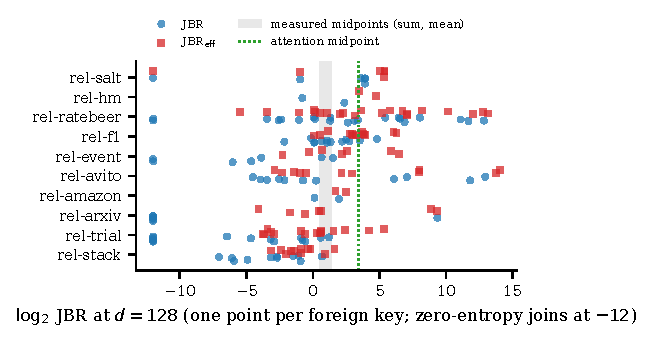
\includegraphics[width=\columnwidth]{relbench_jbr_distribution.pdf}
\caption{$\log_2\jbr$ of all 95 foreign keys of ten RelBench databases at $d = 128$, without (circles) and with (squares) lookup entropy. Gray band: measured sum and mean midpoints; dotted line: attention midpoint.}
\label{fig:real}
\end{figure}

For all 95 foreign keys of ten RelBench databases we computed $K$ (mean number of children of parents with at least one), $H_{\mathrm{row}}$ (sum of plug-in column entropies after discretizing numeric columns into 32 quantile bins and hashing high-cardinality and text columns into 32 buckets, minus each column's shuffle-corrected mutual information with the parent) and $H_{\mathrm{lookup}}$. At $d = 128$ the median ratio is $0.58$ (interquartile range $0.04$ to $5.4$; Fig.~\ref{fig:real}): $44$ foreign keys ($46\%$) exceed $\jbr = 1$, $64$ ($67\%$) when lookup entropy is included, and $34$ at $d = 256$.

For the 30 tasks with published results, we tested whether the ratio predicts RDL difficulty (the within-task-type percentile of the RDL error) or the relative gains of RDL over LightGBM \cite{robinson2024relbench} and of RelGNN \cite{chen2025relgnn} and RelGT \cite{dwivedi2025relgt} over RDL. The pre-specified primary test, entropy-weighted $\jbr_{\mathrm{eff}}$ against RDL difficulty, is null ($\rho = 0.015$, within-database permutation $p = 0.90$, LODO $R^2 = -0.23$). Across all 48 predictor-outcome pairs, ratio-based correlations lie between $-0.25$ and $0.20$ and no test survives Holm correction. Five task-conditional variants, which weight each join by the cross-validated skill of its aggregated features for the label, are also null on 21 entity tasks (all Holm-adjusted $p = 1.0$, all LODO $R^2 < 0$).

\section{Discussion}

\textbf{Reconciling the results.} The controlled experiments and the planted labels show that the bottleneck is real, sharp and predictable. The original tasks show that it rarely binds on current benchmarks. The planted experiment explains why: the same real tables that defeat pooling on query labels are handled perfectly by every aggregator on count labels, and pooling preserves exactly the moments and counts that the original labels appear to depend on. Neighbor sampling also caps $K$ at the fanout, and the standard second layer already supplies the parent-to-child message of Proposition 3. Super-critical joins are therefore common but mostly harmless for today's labels. They become harmful when a prediction depends on whether a specific related record exists, which is common in practice (has this customer bought this product before; has this account logged in from this device), but rare in the benchmark tasks.

\textbf{Design guidance.} For a join whose corrected ratio is well past the transition and whose label may depend on specific child records: send a message from parent to children before pooling and use sum, or use attention with a root term; do not rely on width. For count-like labels, plain sum aggregation is sufficient at any ratio we measured. When using attention in heterogeneous RDL models, keep a root or residual term.

\textbf{Limitations.} The synthetic targets are binary exact-match tasks, and the corrected exponents come from one model family. Planted labels use one column per join, and two of six joins pass the pre-declared inclusion rule; the rule was fixed before the last four joins and the third seed were run, but after the first two joins had been inspected. RelBench runs train on CPUs with budgets below those of published baselines, although a three times longer budget did not change the conclusions. Plug-in entropies on real data are biased for high-cardinality columns.

\section{Conclusion}

Learned pooling at a foreign-key join fails along a sharp, predictable curve. A corrected capacity law, $K H_{\mathrm{row}}^{0.9}/d^{0.2}$, predicts accuracy on unseen joins with $R^2$ near $0.9$; attention and a parent-to-child message move the threshold by about three to four times, and width barely does. The same behavior appears on real RelBench tables when the label depends on a specific child record, but not on the current benchmark tasks, whose labels pooling already preserves. We release all code, the pre-registered predictions and every run record.

\section*{Code and Data Availability}
Code, configurations, pre-registered predictions, run records and analysis outputs are available at \url{https://github.com/vasu-atmakuri/join_bottleneck_ratio_relational_deep_learning}. Every number in this paper is produced by the analysis scripts in that repository.

\setlength{\IEEEbibitemsep}{0pt}\footnotesize
\bibliographystyle{IEEEtran}
\bibliography{references}

\end{document}
